\documentclass[article,12pt]{elsarticle}

\usepackage{graphicx}
\usepackage{booktabs}
\usepackage[utf8]{inputenc}

\usepackage[spanish,es-nodecimaldot,es-tabla]{babel}
\usepackage{csquotes}

\usepackage{amsmath}
\usepackage{amsfonts}

\usepackage[backend=biber, style=apa]{biblatex}
\addbibresource{biblio.bib}
\usepackage{float}

\usepackage{parskip}
\usepackage{url}

\usepackage{float}

% Me da flojera filtrarlos XDD, perdón
\usepackage[spanish]{babel}
\usepackage{amssymb}
\usepackage{flushend}
\usepackage{float}
\usepackage{anysize}
\usepackage{amsmath}
\usepackage{amsfonts}
\usepackage{dcolumn}
\usepackage{amsthm}
\usepackage{caption}
\usepackage{float}
\usepackage{subfigure}
\usepackage{graphicx}
\usepackage{lmodern}
\usepackage{booktabs}
\usepackage{color}
\usepackage{longtable}
\usepackage{rotating}
\usepackage{etoolbox}
\usepackage{comment}
\usepackage{pdflscape}
\usepackage{multicol}
\usepackage{lipsum}
\renewcommand{\theenumi}{\alph{enumi}}

\newfloat{grafica}{htbp}{grf}
\floatname{grafica}{Gráfica}

\renewcommand{\tablename}{Tabla}

\date{05/09/2024}


\begin{document}

%----------------------------------------------------------
    \begin{frontmatter}
    \title{\textbf{Laboratorio de Fenómenos Colectivos} \\  Práctica  I\\ 
        \textit{Relación entre la frecuencia de la resonancia al soplar botellas y el volumen}}
    \author{López González A.$^1$, Hernández Gomez A.$^2$, Villanueva Sanluis A.$^2$, Ornelas Arias C.$^2$}
    \address{$^1$ Facultad de Ciencias, Universidad Nacional Autónoma de México, Apartado Postal 70-399, M\'exico CDMX, 04510, México.}


    \begin{abstract}
    Este trabajo presenta una investigación experimental sobre la relación entre el volumen de recipientes y la frecuencia de resonancia que generan, utilizando botellas de diversas geometrías como cavidades resonantes de Helmholtz. Partiendo de observaciones iniciales que sugieren que la frecuencia del sonido se incrementa al disminuir el volumen de aire, se ha desarrollado un modelo teórico basado en el análisis dimensional y el Teorema de Vaschy-Buckingham. La experimentación involucró la variación del volumen de aire dentro de las botellas mediante el llenado con agua, registrando las frecuencias de resonancia con un método preciso.

Los resultados obtenidos confirman la relación inversamente proporcional entre la frecuencia de resonancia y la raíz cuadrada del volumen de aire, validando tanto el modelo teórico propuesto como la hipótesis inicial. Además, se identificaron pequeñas discrepancias atribuidas a las diferencias geométricas entre los recipientes y las incertidumbres experimentales, las cuales se discuten en el contexto de la precisión de las mediciones. Este estudio no solo ofrece una validación empírica de los principios físicos de resonancia, sino que también proporciona una base sólida para aplicaciones prácticas en el diseño de instrumentos acústicos.
    \end{abstract}

    \begin{keyword}
     Resonador; Helmholtz; Frecuencia; Matraz.
    \end{keyword}
\end{frontmatter}
%----------------------------------------------------------
\begin{multicols}{2}

    \section{Introdución}
        \subsection{Cavidad resonante de Helmholts}
        Es sabido que al soplar con cierta intensidad la boca de una botella podemos hacer que cree una nota característica y además se ha notado que al vertir agua dentro de ella el sonido de agudifica, es de hecho, el principio con el que algunos han creado un objeto musical empleando botellas usadas de casa con solo variar el agua en su interior.
        \\
        En este reporte buscaremos evidenciar experimentalmente la relación que existe entre el volumen de un recipiente y la frecuencia del sonido que produce cuando se le hace resonar. De momento solo sabemos que en medida que se aumenta la cantidad de agua en su interior el sonido emitido al soplar en más agudo, que tentativamente nos indica una relación con el volumen de aire que existe en su interior.

        De acuerdo al análisis que propone el Teorema de Vaschy–Buckingham, para la Cavidad resonante de Helmholtz de volumen V hueco con un cuello de longitud l y diámetro interno \( \phi \). Obtenemos la siguiente relación de frecuencia/propiedades de la botella.
        
        \begin{equation}
         f = \lambda \frac{\upsilon_s}{\sqrt{4^{-1}\pi \phi^2}} \left( \frac{(4^{-1}\pi \phi^2)^2}{lV} \right)^{\xi}
         \end{equation}
        
        En donde \( \xi =  0.45\) para las botellas de geometrías imperfectas y \( \xi = 0.47 \) para el matraz de bola; \(\upsilon_s\) es la velocidad del sonido. Es interesante notar que el único valor cambiante en el desarrollo es el volumen de la botella, además \( 0.45 \approx 0.47 \approx 0.5 \) por lo que tendremos una gráfica muy parecida a \( \frac{\alpha}{\sqrt{x}} \)

        \begin{figure}[H]
        \centering
        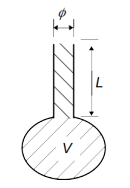
\includegraphics[width = 4cm]{fig1.PNG}
        \caption{Variables geométricas de la botella}
        \end{figure}


        
        
        
\section{Hipótesis}
Creemos que hallaremos una relación exponencial entre el volumen de la botella y la frecuencia de respuesta al soplar, pues se ha observado (en videos de quienes han construído un instrumento mediante este principio) que la relación es no lineal entre notas.


\section{Objetivo}
Obtener la relación matemática entre el volumen de un recipíente, la frecuencia de su sonido, su geometría (largo del cuello, diámetro del interior, curvatura, etc.) y si existiere otro parámetro determinante.


    \section{Procedimiento experimental}
        \subsection{Materiales}
            \begin{itemize}
                \item Vernier
                \item 3 Botellas de vidrio (boing, tehuacán, chaparrita)
                \item Probeta de 250 ml
                \item Matraz de bola de 1000 ml
                \item Celular con app "Sound Level Meter"
            \end{itemize}
        \subsection{Procedimiento}
        Primero, se midió el diámetro interno del cuello de los recipientes estudiados y la longitud de sus cuellos usando el vernier. \\
        A continuación, un miembro del equipo sopló en la orilla del cuello de cada botella vacía para producir un sonido, mientras otro se encargaba de medir la frecuencia del sonido producido usando un dispositivo móvil con la aplicación "Sound Level Meter" en su configuración de incertidumbre más baja (\(\pm 5.4hz\)). Usar esta aplicación consistió en acercar el micrófono del dispositivo al sonido mientras la aplicación lo registraba, en particular se buscó maximizar la curva en una región de las frecuencias, para así obtener la frecuencia natural del sonido producido.\\
        Una vez registrado este dato, se llenó cada botella con distintas cantidades de agua determinadas, y se repitió el proceso descrito previamente, registrando un total de 5 sonidos y sus respectivas frecuencias por cada botella.

    \end{multicols}
    \section{Datos, análisis y discusión de resultados}
    
    \subsection{Datos obtenidos}
    Primero, en la tabla \ref{tab:diam} se presenta el diámetro interno del cuello de cada botella, y la longitud de este.\\

    Es resaltable mencionar que al construir una función que relacione la frecuencia con las características de la botella estos parámetros (diámetro y longitud) serán constantes pues no podemos modificar la geometría de la botella.

    \begin{table*}[h]
    \centering
    \caption{Botellas utilizadas en el experimento, los diámetros internos y las longitudes de sus cuellos }
    \label{tab:diam}
    \begin{tabular}{@{}lll@{}l}
        \toprule
        Botella & Diámetro cuello (cm$\pm 0.01$) & Longitud cuello (cm$\pm 0.05$)  &Volumen (ml $\pm 0.1$)\\ \midrule
        Chaparrita & 1.98 & 8.5  &255\\
        Tehuacán & 1.94 & 4.2  &355\\
        Matraz de bola & 3.65 & 10  &1200\\ \bottomrule
    \end{tabular}
\end{table*}
\\
    
    A continuación, se presentan las tablas \ref{tab:chap}, \ref{tab:tehua} y \ref{tab:matraz} que incluyen la vibración de los sonidos producidos por las distintas botellas con distintos niveles de agua.
    
    \begin{table}[h]
        \centering
        \caption{Frecuencias de sonido medido al hacer vibrar una botella de Chaparrita con distintas cantidades de agua}
        \label{tab:chap}
            \begin{tabular}{@{}ll@{}}
                \toprule
                Agua en la botella (ml$\pm 2.5$) & Frecuencia del sonido (Hz$\pm5.4$) \\ \midrule
                0 & 258 \\
                60 & 301 \\
                120 & 361 \\
                180 & 490 \\
                240 & 1152 \\ \bottomrule
            \end{tabular}%
        \end{table}\\

    \begin{table}[h]
        \centering
        \caption{Frecuencias de sonido medido al hacer vibrar una botella de Tehuacán con distintas cantidades de agua}
        \label{tab:tehua}
            \begin{tabular}{@{}ll@{}}
                \toprule
                Agua en la botella (ml$\pm 2.5$) & Frecuencia del sonido (Hz$\pm5.4$) \\ \midrule
                0 & 172 \\
                80 & 199 \\
                160 & 231 \\
                240 & 323 \\
                320 & 517 \\ \bottomrule
            \end{tabular}%
        \end{table}\\
Para las frecuencias tenemos lo siguiente.
        \begin{table}[h]
        \centering
        \caption{Frecuencias de sonido medido al hacer vibrar un matraz de bola con distintas cantidades de agua}
        \label{tab:matraz}
            \begin{tabular}{@{}ll@{}}
                \toprule
                Agua en la botella (ml$\pm 2.5$) & Frecuencia del sonido (Hz$\pm5.4$) \\ \midrule
                0 & 145 \\
                250 & 161 \\
                500 & 194 \\
                750 & 253 \\
                1000 & 431 \\ \bottomrule
            \end{tabular}%
        \end{table}\\

        Recordemos la ecuación 1.
        \begin{equation*}
         f = \lambda \frac{\upsilon_s}{\sqrt{4^{-1}\pi \phi^2}} \left( \frac{(4^{-1}\pi \phi^2)^2}{lV} \right)^{\xi}
         \end{equation*}

\newpage
        Haciendo la conversión correspondiente de la frecuencia a \textit{Hz}, y del volumen a $m^3$, graficamos $f$ vs $V$ y obtenemos la siguiente figura, en donde incluímos todas las botellas. Hasta ahora todos estos puntos serán disconexos.\\
        Según nuestra hipótesis nuestra gráfica al conectar los puntos debe parecerse aproximadamente a $\frac{\alpha}{\sqrt{x}}$. O más precisamente a $\frac{\alpha}{x^{\xi}}$.
    
        \begin{figure}[H]
        \centering
        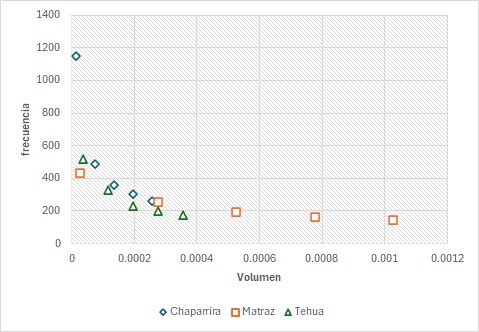
\includegraphics[width = 7cm]{fv.png}
        \caption{Relación Frecuencia-Volumen}
        \end{figure}

        Se ha cumplido la teoría pues el gráfico de $\frac{\alpha}{x^{\xi}}$ para cierto $\alpha$ se comporta igual a nuestro gráfico.
    
    \section{Conclusión}
    A lo largo de este experimento se logró establecer una relación clara entre el volumen de las botellas empleadas y la frecuencia del sonido producido al hacerlas resonar, además se vió que la geometría por la que se rigen (diámetro interno de la boquilla y largo del cuello de la botella) también pueden afectar nuestra frecuencia resultante. Los datos experimentales obtenidos muestran que a medida que disminuye el volumen de aire dentro del recipiente, la frecuencia de resonancia aumenta, lo que concuerda con la predicción teórica basada en el análisis dimensional de la Cavidad Resonante de Helmholtz.
    El comportamiento no lineal observado en las gráficas de frecuencia versus volumen confirma que la relación puede modelarse adecuadamente mediante una función inversamente proporcional a aproximadamente la raíz cuadrada del volumen, o más precisamente.
    \begin{equation*}
         f = \lambda \frac{\upsilon_s}{\sqrt{4^{-1}\pi \phi^2}} \left( \frac{(4^{-1}\pi \phi^2)^2}{lV} \right)^{\xi}
         \end{equation*}
    Lo que se ajusta a las predicciones teóricas derivadas de la ecuación de resonancia. Esta concordancia entre teoría y experimento valida nuestra hipótesis inicial.
    
    Además, las pequeñas discrepancias entre los resultados obtenidos para las distintas botellas pueden atribuirse a las diferencias geométricas y posibles imprecisiones experimentales, como la variabilidad en la medición de las frecuencias o en la homogeneidad del flujo de aire al soplar. Sin embargo, dentro de los márgenes de incertidumbre considerados, los resultados son consistentes y refuerzan la relación teórica esperada entre el volumen de aire y la frecuencia de resonancia.
    
    \section{Bibliografía}

G. K. Batchelor, An Introduction to Fluid Dynamics, Cambridge University Press, 2000.

A. Hirschberg, A. van Steenhoven, and A. R. de Jong, "Aeroacoustics of wind instruments," Journal of Sound and Vibration, vol. 143, no. 1, pp. 1-35, 1990.

T. M. McKinsey, "Sound propagation in turbulent air," The Journal of the Acoustical Society of America, vol. 118, no. 5, pp. 2388-2395, 2005.

D. H. Keefe, "Acoustical wave propagation in cylindrical ducts: Transmission line parameter approximations for isothermal and non-isothermal boundary conditions," The Journal of the Acoustical Society of America, vol. 75, no. 1, pp. 58-62, 1984.

A. R. Kergomard and D. Boubenec, "Helmholtz resonators: Theoretical and experimental analysis of the linear regime," The Journal of the Acoustical Society of America, vol. 132, no. 4, pp. 2618-2625, 2012.

M. J. Lighthill, "On sound generated aerodynamically. I. General theory," Proceedings of the Royal Society A, vol. 211, pp. 564-587, 1952.

F. H. Rayleigh, The Theory of Sound, Dover Publications, 1945.

E. G. Kinsler, A. R. Frey, A. B. Coppens, and J. V. Sanders, Fundamentals of Acoustics, 4th ed., John Wiley & Sons, 1999.

\end{document}
